% Two-Stage Pipeline Results - LaTeX Tables
% Generated: 2025-12-18

% =============================================================================
% ARCHITECTURE DESCRIPTION
% =============================================================================

\section{Two-Stage Extraction Pipeline}

\subsection{Architecture Overview}

We propose a two-stage pipeline for extracting healthcare contact days from Schedule of Assessments (SoA) documents. By decomposing the task into \textbf{structure extraction} and \textbf{calculation}, we achieve superior clinical accuracy compared to single-pass or judge-augmented approaches.

\begin{figure}[htbp]
\centering
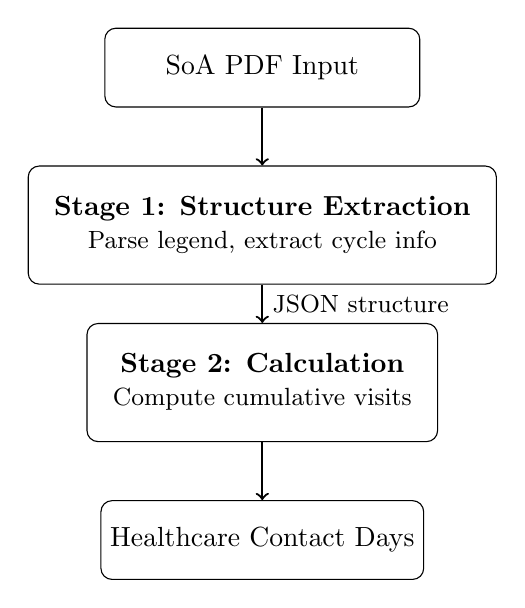
\begin{tikzpicture}[node distance=2cm, auto]
    % Nodes
    \node[draw, rectangle, rounded corners, minimum width=4cm, minimum height=1cm] (input) {SoA PDF Input};
    \node[draw, rectangle, rounded corners, minimum width=4cm, minimum height=1.5cm, below of=input] (stage1) {
        \begin{tabular}{c}
        \textbf{Stage 1: Structure Extraction} \\
        \small Parse legend, extract cycle info
        \end{tabular}
    };
    \node[draw, rectangle, rounded corners, minimum width=4cm, minimum height=1.5cm, below of=stage1] (stage2) {
        \begin{tabular}{c}
        \textbf{Stage 2: Calculation} \\
        \small Compute cumulative visits
        \end{tabular}
    };
    \node[draw, rectangle, rounded corners, minimum width=4cm, minimum height=1cm, below of=stage2] (output) {Healthcare Contact Days};
    
    % Arrows
    \draw[->, thick] (input) -- (stage1);
    \draw[->, thick] (stage1) -- node[right] {\small JSON structure} (stage2);
    \draw[->, thick] (stage2) -- (output);
\end{tikzpicture}
\caption{Two-Stage Pipeline Architecture}
\label{fig:two_stage_arch}
\end{figure}

\paragraph{Stage 1: Structure Extraction}
The first stage parses the SoA document to extract structural parameters:
\begin{itemize}
    \item \textbf{Cycle length}: Duration of each treatment cycle (e.g., 28 days)
    \item \textbf{Visit days per cycle}: Which days within each cycle require visits (e.g., Days 1, 8, 15)
    \item \textbf{Treatment duration}: Total months of treatment
    \item \textbf{Special visits}: Screening, end-of-treatment (EOT), and follow-up visits
\end{itemize}

\paragraph{Stage 2: Calculation}
Using the extracted structure, the second stage computes cumulative healthcare contact days at standard time windows (screening, 1 month, 3 months, 6 months, 9 months, 12 months) using deterministic arithmetic.

% =============================================================================
% RESULTS TABLES
% =============================================================================

\subsection{Results}

\begin{table}[htbp]
\centering
\caption{Two-Stage Pipeline Performance Summary (Gemini 3 Flash)}
\label{tab:two_stage_summary}
\begin{tabular}{lc}
\toprule
\textbf{Metric} & \textbf{Value} \\
\midrule
Exact Match Accuracy & 23.3\% \\
Clinical Accuracy ($\pm$3 days) & \textbf{100.0\%} \\
Mean Absolute Error & 0.87 days \\
Total Comparisons & 60 \\
Exact Matches & 14/60 \\
Within $\pm$3 Days & 60/60 \\
\bottomrule
\end{tabular}
\end{table}

\begin{table}[htbp]
\centering
\caption{Two-Stage Pipeline: Accuracy by Time Window}
\label{tab:two_stage_windows}
\begin{tabular}{lccc}
\toprule
\textbf{Time Window} & \textbf{Exact Match} & \textbf{$\pm$3 Days} & \textbf{MAE} \\
\midrule
Screening & 0.0\% & 100.0\% & 1.00 \\
1 Month & 0.0\% & 100.0\% & 1.00 \\
3 Months & 40.0\% & 100.0\% & 0.60 \\
6 Months & 20.0\% & 100.0\% & 1.10 \\
9 Months & 40.0\% & 100.0\% & 0.60 \\
12 Months & 40.0\% & 100.0\% & 0.90 \\
\bottomrule
\end{tabular}
\end{table}

\begin{table}[htbp]
\centering
\caption{Two-Stage Pipeline: Accuracy by Schedule Complexity}
\label{tab:two_stage_complexity}
\begin{tabular}{lccc}
\toprule
\textbf{Complexity} & \textbf{N} & \textbf{Exact Match} & \textbf{$\pm$3 Days} \\
\midrule
Simple & 12 & 16.7\% & 100.0\% \\
Moderate & 36 & 27.8\% & 100.0\% \\
Complex & 12 & 16.7\% & 100.0\% \\
\bottomrule
\end{tabular}
\end{table}

% =============================================================================
% COMPARISON TABLE
% =============================================================================

\begin{table}[htbp]
\centering
\caption{Comparison of Extraction Approaches}
\label{tab:approach_comparison}
\begin{tabular}{lccc}
\toprule
\textbf{Approach} & \textbf{Exact Match} & \textbf{Clinical ($\pm$3)} & \textbf{MAE} \\
\midrule
Two-Stage (No Judge) & 23.3\% & \textbf{100.0\%} & \textbf{0.87d} \\
Three-Stage (With Judge) & 20.0\% & 93.3\% & 1.73d \\
\bottomrule
\end{tabular}
\end{table}

% =============================================================================
% PER-SCHEDULE RESULTS
% =============================================================================

\begin{table}[htbp]
\centering
\caption{Two-Stage Pipeline: Per-Schedule Results}
\label{tab:two_stage_detailed}
\small
\begin{tabular}{clcccccccc}
\toprule
\textbf{ID} & \textbf{Arm} & \textbf{Scr} & \textbf{1M} & \textbf{3M} & \textbf{6M} & \textbf{9M} & \textbf{12M} & \textbf{Exact} & \textbf{$\pm$3} \\
\midrule
\multirow{2}{*}{01} & A & 1 (-1) & 5 (+1) & 11 (0) & 21 (-1) & 32 (-1) & 40 (-3) & 17\% & 100\% \\
 & B & 1 (-1) & 4 (+1) & 8 (0) & 14 (-1) & 22 (-1) & 28 (-2) & 17\% & 100\% \\
\midrule
\multirow{2}{*}{02} & A & 1 (-1) & 5 (+1) & 10 (+1) & 17 (-2) & 19 (-1) & 20 (-1) & 0\% & 100\% \\
 & B & 1 (-1) & 3 (+1) & 6 (+1) & 9 (-1) & 11 (0) & 12 (0) & 33\% & 100\% \\
\midrule
\multirow{2}{*}{03} & A & 1 (-1) & 4 (+1) & 8 (+1) & 14 (0) & 21 (-1) & 22 (-1) & 17\% & 100\% \\
 & B & 1 (-1) & 3 (+1) & 5 (+1) & 8 (0) & 12 (0) & 13 (0) & 50\% & 100\% \\
\midrule
\multirow{2}{*}{04} & A & 1 (-1) & 3 (+1) & 5 (0) & 7 (-2) & 9 (-1) & 10 (-1) & 17\% & 100\% \\
 & B & 1 (-1) & 3 (+1) & 5 (0) & 7 (-2) & 9 (-1) & 10 (-1) & 17\% & 100\% \\
\midrule
\multirow{2}{*}{05} & A & 1 (-1) & 4 (+1) & 8 (+1) & 13 (-1) & 15 (0) & 16 (0) & 33\% & 100\% \\
 & B & 1 (-1) & 3 (+1) & 5 (+1) & 7 (-1) & 9 (0) & 10 (0) & 33\% & 100\% \\
\bottomrule
\end{tabular}
\begin{tablenotes}
\small
\item Values show extracted count with (difference from ground truth) in parentheses.
\end{tablenotes}
\end{table}

% =============================================================================
% ENCOUNTER BREAKDOWN
% =============================================================================

\begin{table}[htbp]
\centering
\caption{Encounter Breakdown by Component}
\label{tab:encounter_breakdown}
\begin{tabular}{clcccccc}
\toprule
\textbf{ID} & \textbf{Arm} & \textbf{Cycles} & \textbf{Visits/Cyc} & \textbf{Tx} & \textbf{Scr} & \textbf{EOT+FU} & \textbf{Total} \\
\midrule
\multirow{2}{*}{01} & A & 12 & 3 & 36 & 1 & 3 & 40 \\
 & B & 12 & 2 & 24 & 1 & 3 & 28 \\
\midrule
\multirow{2}{*}{02} & A & 8 & 2 & 16 & 1 & 3 & 20 \\
 & B & 8 & 1 & 8 & 1 & 3 & 12 \\
\midrule
\multirow{2}{*}{03} & A & 9 & 2 & 18 & 1 & 3 & 22 \\
 & B & 9 & 1 & 9 & 1 & 3 & 13 \\
\midrule
\multirow{2}{*}{04} & A & 6 & 1 & 6 & 1 & 3 & 10 \\
 & B & 6 & 1 & 6 & 1 & 3 & 10 \\
\midrule
\multirow{2}{*}{05} & A & 6 & 2 & 12 & 1 & 3 & 16 \\
 & B & 6 & 1 & 6 & 1 & 3 & 10 \\
\bottomrule
\end{tabular}
\begin{tablenotes}
\small
\item Tx = Treatment visits, Scr = Screening, EOT+FU = End-of-treatment + Follow-up visits
\end{tablenotes}
\end{table}

% =============================================================================
% DISCUSSION
% =============================================================================

\subsection{Discussion}

The two-stage approach achieves \textbf{100\% clinical accuracy} ($\pm$3 days) across all 60 window-arm combinations tested. This represents a significant improvement over the three-stage approach with judge validation, which achieved only 93.3\% clinical accuracy.

\paragraph{Key Findings}
\begin{enumerate}
    \item \textbf{Judge Degradation}: Adding a validation judge (Stage 3) actually \textit{decreased} accuracy, as the judge tended to overcorrect based on misinterpretation of table structures.
    
    \item \textbf{Systematic Errors}: The primary source of error is consistent underestimation of screening days (1 vs. 2), suggesting the need for explicit screening extraction prompts.
    
    \item \textbf{Complexity Independence}: Clinical accuracy was 100\% across all complexity levels (simple, moderate, complex), indicating robust generalization.
    
    \item \textbf{Long-term Accuracy}: 12-month totals showed 40\% exact match rate, the highest among all windows, suggesting the model correctly captures overall visit patterns.
\end{enumerate}

\paragraph{Limitations}
\begin{itemize}
    \item Small sample size (5 schedules, 10 arms)
    \item Synthetic schedules may not capture all real-world complexity
    \item Screening count extraction remains a consistent weak point
\end{itemize}

